\section{Versuchsaufbau}
%skizze zum versuchsaufbau (oder foto) einf�gen,   es muss erkl�rt werden wie das ganze funktioniert und welche speziellen einstellungen verwendet wurden (z.b. welche kn�pfe an den ger�ten f�r die messung verdreht wurden)
Bei dem SQUID handelt es sich um ein rf-SQUID, welches auf einem Yttrium-Barium-Kupferoxid (YBa$_2$ Cu$_3$ O$_7$) Supraleiter basiert. Der Supraleiter ist ein Supraleiter 2. Art und hat eine Sprungtemperatur von T$_c$ = 92K. F�r die K�hlung wird fl�ssiger Stickstoff verwendet. Der Supraleiter und der fl�ssige Stickstoff befinden sich in einem Dewar-Gef�� zur thermischen Isolation. Das Dewar-Gef�� ist von mehren Zylindern zur Abschirmung umgeben. Zur Abschirmung werden Aluminium und $\mu$-Metall verwendet. Die Zylinder sind noch von eine Metalltonne umgeben, welche �ber einen Seilzug angehoben werden kann. Alle Abschirmungen sind an eine Erdung angeschlossen.
F�r die Eichung des SQUID ist ein Schlitten unterhalb des Dewar-Gef�� angebracht, mit dem eine Leiterschleife mittig unter dem Sensor angebracht werden kann. Mit dem Schlitten k�nnen auch noch andere Objekte unterhalb des Detektors in Position gebracht werden.
Das SQUID l�sst sich �ber ein Toutch-Panel steuern, die Messdaten werden �ber ein Oszilloskop ausgegeben. Ein schematische Aufbau ist in Abb.\ref{fig:schem_auf} zu sehen.

\begin{figure}[H]
\centering
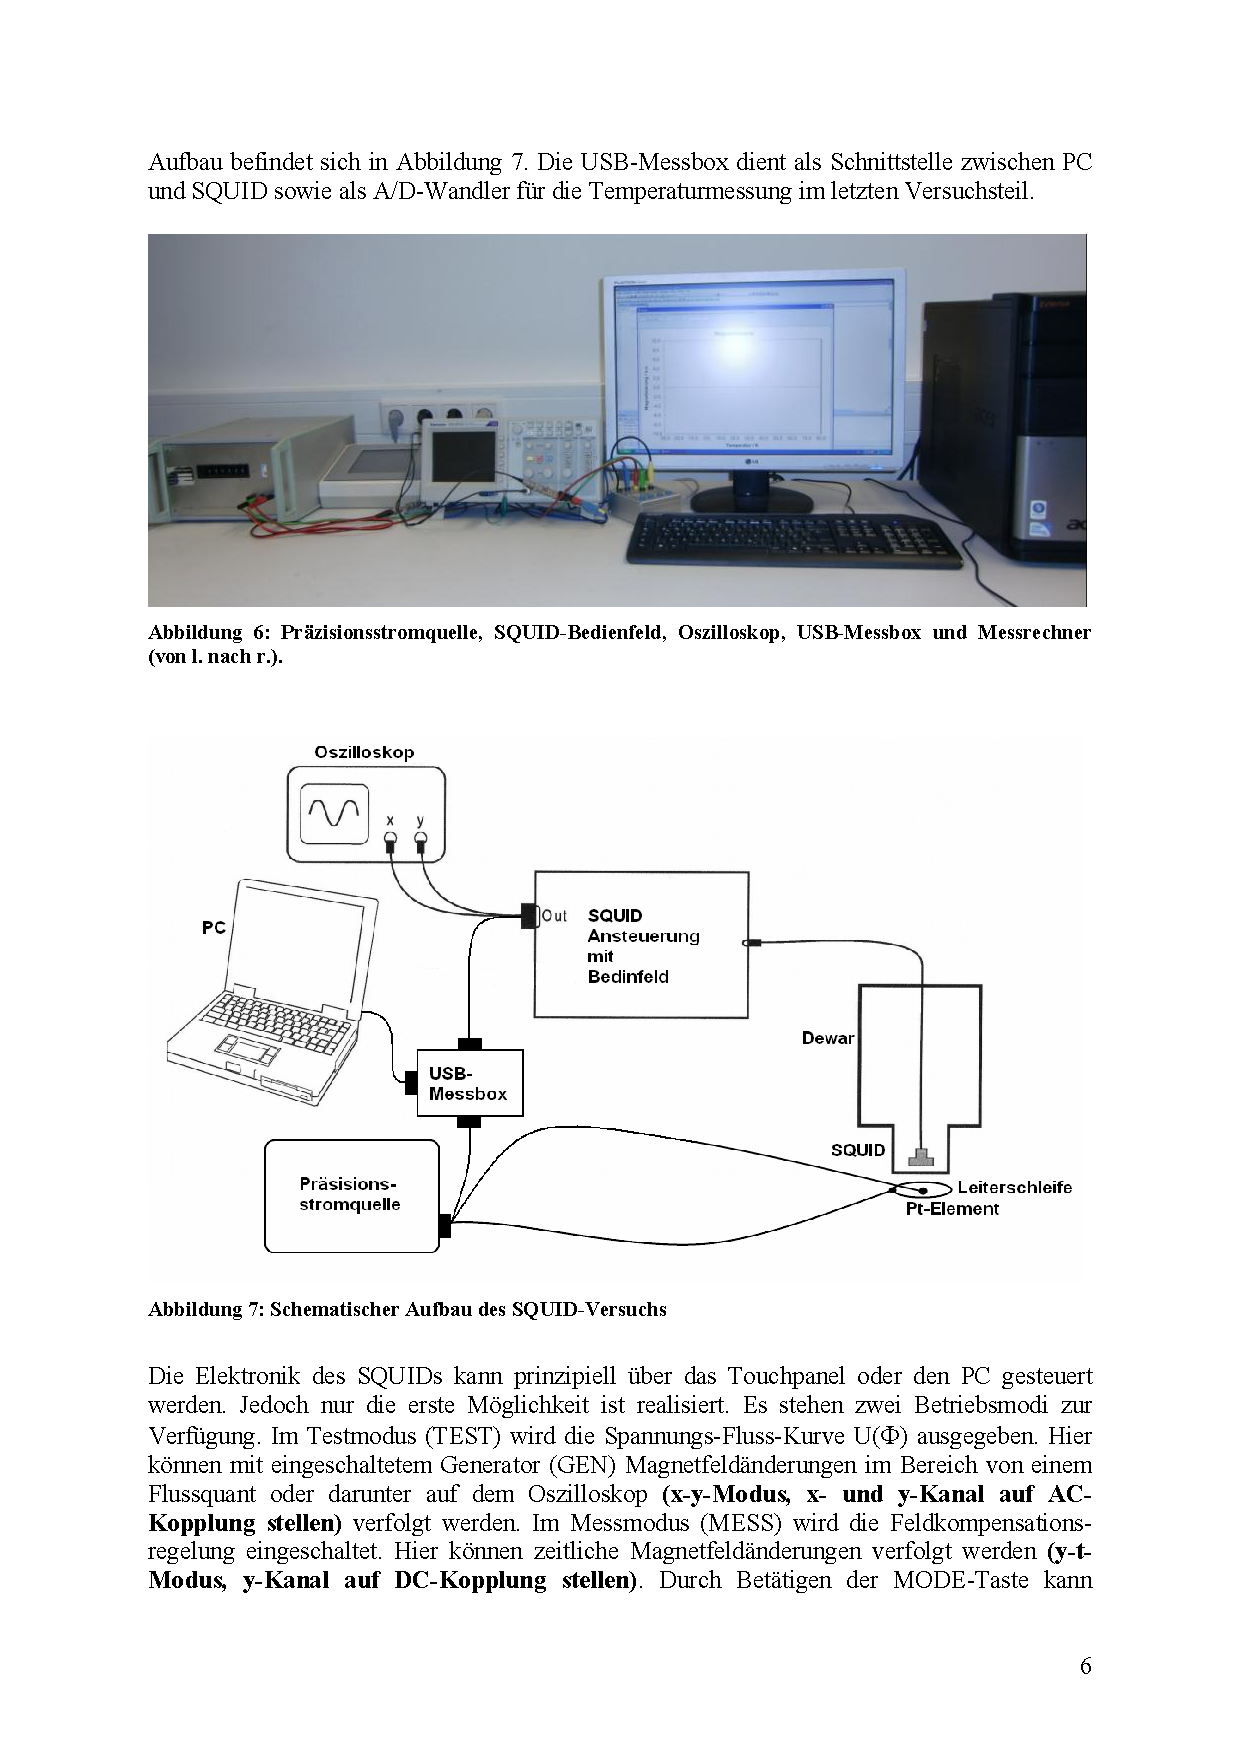
\includegraphics[scale = 1,trim = 10mm 80mm 10mm 120mm, clip]{aufbau_1}
\caption{Aufbau des Experiments \cite{Schematischer_Aufbau}}
\label{fig:schem_auf}
\end{figure}